\chapter{Introduction}
\markboth{Introduction}{}
\label{ch:introduction}

\begin{fquote}[Henry Nix] Data does not equal information; 
information does not equal knowledge; and, most importantly 
of all, knowledge does not equal wisdom. We have oceans of data, 
rivers of information, small puddles of knowledge, and 
the odd drop of wisdom. \fqsource{{Keynote address, AURISA, 1990}} \end{fquote}


\begin{synopsis}
This chapter conceptualises the topic of this dissertation
with respect to the methodology and application. The chapter
also covers the motivations for research, contributions of the thesis %and also contributions of the thesis 
to the scientific community, and organisation of the chapters
of the thesis.
\end{synopsis}

\section{Data Explosion}
\label{s:data}

Dictionary definition of data is a piece of information that ranges from 
the values or measurements of quantitative and qualitative variables
to the description of objects or phenomenon~\cite{merriam02}. In computing 
terms, data is any digitally stored information. Throughout history,
data was universal, and found everywhere. However, only employees generated 
data in computing terms by keying in the handwritten information. Nowadays, 
users generate data on their own, for example, social network statuses 
or photos, thereby increasing the amount of data produced. Furthermore, new 
machines such as automatic climatic conditions recorder and technologies such 
as Large Hadron Col\-lid\-er (LHC) produce colossal amount of data~\cite{lynch08}. 
This astronomical increase in the amount of data is ref\-erred to as big 
data~\cite{lynch08,manyika11frontier}. Modern 
science revolves around the methods and ways to analyse the data generated 
in their field to stimulate scientific discoveries. 
%Nowadays, data driven methods 
%have been use to stimulate new discoveries. 

Production of data these days is such humongous that it surpasses the 
estimates of Moore's Law~\cite{moore1965}. For example, 5 exabytes (EB)
(1 EB= $10^{18}$ bytes = 1 billion gigabytes) of data was generated 
from  the dawn of civilisation until 2003. Today, we create 5EB of data 
every two days~\cite{sagiroglu13}. Three properties: Volume, Velocity, 
and Variety  (often referred to by 3Vs) define the big data. The 
volume of data and speed at which they arrive and leave the real time 
systems provide challenges in big data analysis. In addition, variety 
in the collected data also poses considerable challenges to research in  
big data. 

Over the years, measurement technology has progressed enormously, and 
produces variety of data in addition to the large volumes of data 
because each cycle of improvement in measurement technology produces 
data in a different representation. The variety is the aspect of big  
data that is closest to the topic of this thesis. Nowadays, 
individual dataset in the sets of datasets often have higher 
dimensionality, $d$, than the number of samples, $N$, i.e., $d\gg N$. 
Therefore, challenge in big data analysis is large temporal, 
and/or spatial data dimensions which results in the curse of 
dimensionality~\cite{bellman61}. Traditional %machine learning and data mining 
algorithms succumb to the challenges posed
by small sample high dimensional datasets. Therefore, it is
imperative to develop novel methods to analyse multiple datasets, 
i.e., sets of datasets in different representations within 
a single analysis.



Biology is one of the largest producer of big data
which necessitates novel computational methods to analyse 
such wealth of data and to convert data to knowledge and 
wisdom~\cite{howe08,marx2013}. There are varieties of biological 
phenomena often interlinked with one another making variety
aspect of big data prevalent in biological data source.
This tremendous increase in biological data coupled with 
the variety is impossible to interpret using visual analysis. 
Instead, it requires novel computational methods for thorough
understanding of the biological phenomenon. The growth of
biological data has produced both opportunities and challenges 
for researchers to develop algorithms  and analysis methods
in computational domain to extract biological meaning from 
vast amounts of data.


\section{Machine Learning and Data Mining}
\label{s:mldm}

Machine Learning is a core sub--area of artificial intelligence that
intersects the discipline of computer science, and statistics. The aim of 
machine learning  is to develop algorithms that learn from the observed data, and use 
the experience to improve the performance~\cite{barberBRML12,bishop06,hastie09,mitchell97}.
Machine learning includes a myriad of statistical, probabilistic and 
optimisation, and induction algorithms that are applicable in different 
tasks such as classification, regression, clustering, and pattern 
discovery. Data mining, also known as knowledge discovery, is the 
process of extracting useful information such as patterns, from 
unstructured and enormous sets of data by analysing data from different
perspectives~\cite{hand01}.

Machine learning and data mining complement each other and 
it is difficult to make a clear distinction between the two. 
Nonetheless,
machine learning algorithms are often used in the data mining 
process. Machine learning and data mining, although a new 
discipline, has a large active research community. The community
has already  developed a cohort of fascinating algorithms and 
methods to treat  the concept classes, and elegant and clever 
ways to search through  databases. Hence, machine learning 
and data mining methods can address the challenges posed by 
data intensive disciplines such as biology.


In application areas such as biology, the number of training 
samples are often limited even in the age of big data. In contrast,
the data dimensionality increases considerably. For example, in 
genetics, number of cancer patients is constant while the new 
technology  can measure the finer units of the phenomenon generating 
data with large dimensionality. The implication of increasing 
dimensionality is that, with a limited size of training samples, 
the performance of the algorithm deteriorates as the number of 
features increases. This phenomenon is also called Hughes 
phenomena, or Hughes effect~\cite{hughes68} or more generally
as a curse of dimensionality~\cite{bellman61}.

\subsection{Mixture Model}
\label{ss:mixmdl}

A mixture model is a probabilistic modelling technique 
in machine learning and data mining community which models a 
data distribution under the assumption that all the data points 
are generated from a mixture of parametric probability 
distributions~\cite{bishop06,everittmixdist,mclachlanfmm}. 
Apart from this assumption of data origination, mixture models
are flexible probabilistic models with varying uses
such as model based clustering, classification, image analysis,
and collaborative filtering in analysis of high dimensional data.
Mixture models are suitable for the choice of any probability
distributions such as the Gaussian, Bernoulli, Poisson, and
Dirichlet. In this thesis, mixture models analyse multiresolution 
data probabilistic clustering setting.  Chapter~\ref{ch:mixmodels} 
discusses mixture models in detail.

\section{Challenges of Multiresolution Data}
\label{s:multiresdata}

Measurement of physical phenomenon such as distance, weight, and time
started since the time immemorial and has been the cornerstone of our 
knowledge and learning~\cite{klein2012science}. Measurement has also
become integral part of our everyday life. The inventions and discoveries 
of the modern world would cease to exist in absence of measurement 
technology. The measurement technology has been continuously improving 
over the years. Result of a measurement process is generation of the 
data. The older generation technologies measure only the coarser unit of the 
phenomenon generating data in coarse resolution. In contrast, the newer 
generation technologies measure the finer units of the phenomenon  
producing the data in fine resolution~\cite{measureimprove,Garland99,mardis2011}. 
Resolution here defines the amount of information in each data sample, 
i.e., the level of detail.

%The coarse units contains lesser information 
%while the fine units consists of more information. 

Multiresolution data is generated when the same phenomenon is
measured in different levels of detail~\cite{barth2002multiscale,Garland99,willsky02}. 
Thus, the multiresolution data describes the same phenomenon in 
different data representations. Different data representation is 
a broader challenge in machine learning and data mining community 
where datasets are represented in different forms such as audio, 
video, image, table, and text. This thesis concentrates on 
different data representation only in the context of dimensionality, 
i.e., datasets are same except for the data dimensionality. 
Nevertheless, the proposed algorithms and methods can possibly
be extended to other different data representations. The measurement
of time is one of the simplest illustrations of multi\-resolution 
data. We can measure time in fine units such as seconds and minutes
producing data at a fine resolution. In contrast, we can also measure 
time in coarse units such as months, and years producing data in coarse
resolution. 


\begin{figure}[h!]
\centering
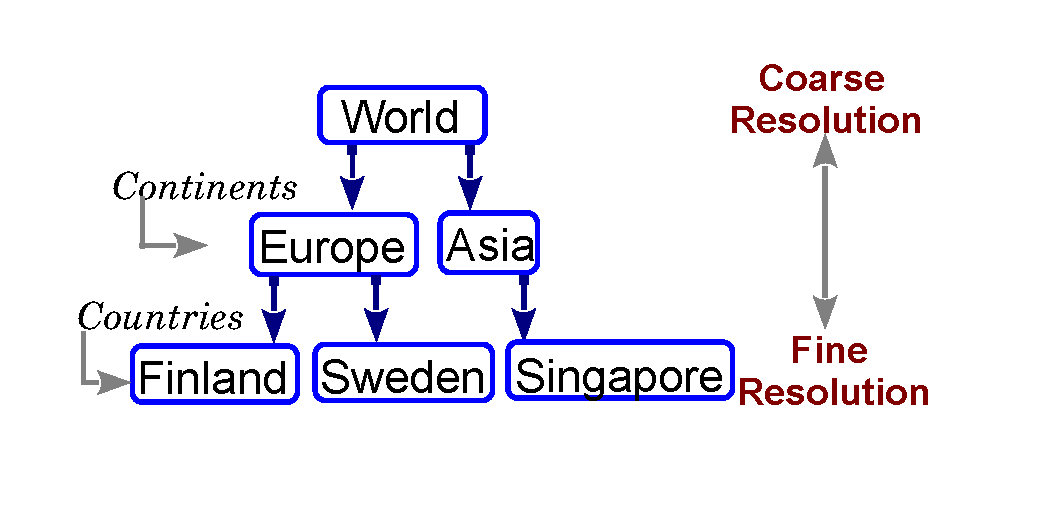
\includegraphics[trim=15mm 20mm 22mm 2mm,width=0.99\textwidth]{figures/oncology}
\caption[Example of Part of Hierarchy.] {Example of part of hierarchy in
real world scenario. The figure shows the geographical division as 
the part of hierarchy which when measured results in multiresolution 
data. The world is divided into continents and continents into countries.} 
\label{Fig:oncology}
\end{figure}

Multiresolution data often forms a part of hierarchy as shown in 
Figure~\ref{Fig:oncology}. For example, the world is a collection
of different continents such as Asia, Europe, and Africa. This 
generates coarser view of data. Similarly, the world is also a 
collection of different countries such as Singapore, Finland, 
and Sweden. These countries can be grouped into different 
continents. Furthermore, these countries can be divided into 
municipalities, and the municipalities into streets, and the 
streets into blocks. This hierarchy forms a multiresolution 
data which represents a part of hierarchy~\cite{russell1911}. 
This division of the world is just an illustrative example, 
as the sources of multiresolution data are varied, for example, 
telecommunications, hydrology, and biology~\cite{willsky02}.
Chapter~\ref{ch:analysismultires} discusses multiresolution 
biological data used in the experiments of the thesis.



\section{Contributions of the Thesis}
\label{s:contributions}

This thesis addresses an important challenge encountered in data analysis:
what should be done when the data to be analysed are represented differently. 
The thesis presents different frameworks and methods amalgamating probabilistic 
modelling and pattern mining domain. The presented methods handle 
irregular, and heterogeneous division of data in different
representations. The major scientific contributions in this thesis are 
summarised in the following list.

\begin{itemize}
 \item Different deterministic data transformation methods are proposed 
 to transform the multiresolution datasets from one resolution to another. 
 The transformed datasets in same resolution can be integrated and modelled 
 in same resolution. 

 \item A computationally  efficient algorithm is proposed to train a series
 of mixture models to aid model selection. The trained mixture models in the
 series differ in number of components but are otherwise similar to each 
 other. This provides an effective means to compare different model selection 
 criteria such as likelihood, AIC, and BIC using different model selection
 techniques such as cross--validation.

 \item A mixture modelling solution is proposed to model multiresolution 
 data by merging the mixture components of different mixture models in 
 different resolutions. The proposed mixture modelling solution initially 
 trains a mixture model in each resolution and merges the similar  
 mixture components across different resolutions to incorporate information 
 in multiple resolutions.

 \item An algorithm that uses domain ontology, known apriori, to determine 
 multiresolution mixture components of the mixture model is proposed to 
 build a single mixture model for multiresolution data. Each individual 
 mixture component is a fully functional Bayesian network.
  %comprehensively 
 \item A three part methodology is proposed to analyse the multi\-resolution
 data blending clustering using mixture models, pattern mining using semantic
 data mining, and visualisation using banded matrices.
 
\end{itemize}

\section{Organisation of the Thesis}
\label{s:organization}
The thesis consists of two parts: an introductory part consisting of 
six different chapters and publications. 
In the introductory part, this chapter introduces the research domain, 
and the Chapter~\ref{ch:analysismultires} 
introduces multiresolution data with a focus on cancer genomics,
and reviews the previous work in multiresolution analysis and 
the related areas. Chapter~\ref{ch:mixmodels} describes mixture 
models and model selection in mixture models. It also 
summarises our contribution for efficient training of a series of 
mixture models~(\citepub{j1}). 

Chapter~\ref{ch:multiresmodel} forms the crux of this thesis and 
discusses  our contributions in multiresolution modelling. First,  
multiresolution data is modelled using deterministic data transformation 
methods for data integration~(\citepub{c1}). Second, multiresolution 
data is modelled by merging the similar mixture components of different 
mixture models  in different resolutions. The merging of mixture 
components models the interaction between the models in different data 
resolutions~(\citepub{c2}). Third, a multiresolution mixture model 
having multiresolution mixture components is proposed to analyse 
the multiresolution data with a single mixture model. Structure
of multiresolution components is  known from the domain 
ontology~(\citepub{c3}). Finally, a comprehensive solution for the 
analysis of multiresolution data is provided using three part 
methodology comprising of clustering, semantic pattern mining, 
and banded matrices~(\citepub{j2}). Chapter~\ref{ch:summary} 
summarises the findings, presents the conclusions of the research, 
and also outlines the possible future work related to the topic of 
the thesis. 

%can generate research
%challenges for machine learning and data mining community.

%Overwhelming amount of data is produced in any fields of science 
%in the world. 


%In summary, the thesis presents different framework and methods 
%amalgamating probabilistic modelling and pattern mining domain. 
%The presented methods handles 
%irregular, inconsistent, and heterogeneous division of regions.
%The developed 
%framework and methods analyzes and models the multiresolution chromosomal 
%amplification datasets with plausible results. 
% The main aim 
%of the thesis the development of models and methods to analyze multiresolution 
%data within a single analysis. 
%solution for the multiresolution data. 
%Each component of the mixture model represents the multiresolution structure
%of the data determined from the domain ontology. 




%The contributions of 
%the dissertation can be summarized with the contributions in \citepub{c1}
%\section{Multiresolution Data}
%\label{s:multiresdata}
%Multiresolution data is generated when the same phenomena is measured 
%with different levels of precision. 
%\section{Multiresolution Data}
%\label{s:multiresdata}
%developed framework and methods analyzes and models the multiresolution 
%chromosomal amplification datasets.
%, i.e., features such 
%as the pyramid structure in image processing domain~\cite{wilson00}. 


%The overall contribution of this thesis is the presentation of novel framework 
%and methods for the analysis of multiresolution data within a single analysis.
%The motivating challenge covered in the thesis comes from the bioinfomatics 
%where chromosomal application patterns of cancer patients are represented in 
%different resolutions. The thesis presents different framework and methods 
%amalgamating probabilistic modelling and pattern mining domain. The developed 
%framework and methods analyzes and models the multiresolution chromosomal 
%amplification datasets with plausible results. The presented methods handles 
%irregular, inconsistent, and heterogeneous division of regions. The main aim 
%of the thesis the development of models and methods to analyze multiresolution 
%data within a single analysis. 

%\citepub{c1} presents deterministic data transformation methods to transform 
%the datasets from one resolution to another providing an opportunity to integrate 
%datasets in different resolutions. The transformed data and the data in the same 
%resolutions are integrated analogous to data integration methods. The resulting 
%integrated data can then be modeled in a single resolution. Similarly, \citepub{j1} 
%pro\-vides a computationally  efficient method to train a series of mixture models 
%to aid model selection. The trained mixture models in the series differ in number 
%of components but are otherwise similar to each other thus providing an effective 
%method for model selection. 


%\citepub{c2} provides a mixture modelling solution to multiresolution data
%by merging of mixture components of different mixture models in different 
%resolutions. The proposed mixture modelling solution  initially trains 
%mixture model in each resolution and merges the similar  mixture components 
%across different resolutions to incorporate information in the multiple 
%resolution. Furthermore, \citepub{c3} provides a single mixture modelling 
%solution for the multiresolution data. Each component of the mixture model 
%represents the multiresolution structure of the data
%determined from the domain ontology. The individual mixture components
%are fully functional Bayesian networks. Finally, \citepub{j2} proposes
%a comprehensive analysis of real world multiresolution data blending clustering 
%using mixture models, pattern mining using semantic data mining, and
%visualization using banded matrices.

%In fact, data science  has emerged as one of the best 
%choice for future career options in recent times~\cite{davenport2012}. 